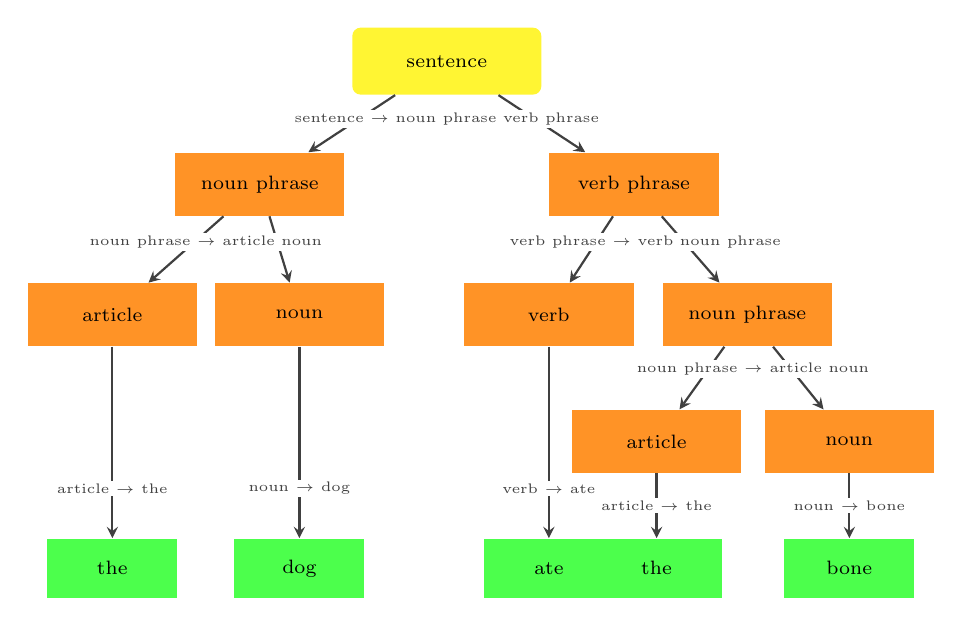
\begin{tikzpicture}[
    x=0.72cm, y=0.92cm,
    >=stealth,
    arr/.style={->, thick, draw=black!75},
    ntbox/.style={draw=none, fill=orange!85, minimum width=2.15cm,
        minimum height=0.8cm, align=center, font=\scriptsize},
    topbox/.style={draw=none, fill=yellow!80, rounded corners=3pt,
        minimum width=2.4cm, minimum height=0.85cm, align=center, font=\scriptsize},
    termbox/.style={draw=none, fill=green!70, minimum width=1.65cm,
        minimum height=0.75cm, align=center, font=\scriptsize},
    rulelabel/.style={font=\tiny, fill=white, inner sep=1pt,
        text=black!75, align=center}
]

\node[topbox] (sentence) at (10.5,7.25) {sentence};

\node[ntbox] (np1) at (7.2,5.55) {noun phrase};
\node[ntbox] (vp)  at (13.8,5.55) {verb phrase};

\node[ntbox] (art1)  at (4.6,3.75) {article};
\node[ntbox] (noun1) at (7.9,3.75) {noun};
\node[ntbox] (verb)  at (12.3,3.75) {verb};
\node[ntbox] (np2)   at (15.8,3.75) {noun phrase};

\node[ntbox] (art2)  at (14.2,2.0) {article};
\node[ntbox] (noun2) at (17.6,2.0) {noun};

\node[termbox] (the1) at (4.6,0.25) {the};
\node[termbox] (dog)  at (7.9,0.25) {dog};
\node[termbox] (ate)  at (12.3,0.25) {ate};
\node[termbox] (the2) at (14.2,0.25) {the};
\node[termbox] (bone) at (17.6,0.25) {bone};

\draw[arr] (sentence) -- (np1);
\draw[arr] (sentence) -- (vp);

\draw[arr] (np1) -- (art1);
\draw[arr] (np1) -- (noun1);

\draw[arr] (vp) -- (verb);
\draw[arr] (vp) -- (np2);

\draw[arr] (np2) -- (art2);
\draw[arr] (np2) -- (noun2);

\draw[arr] (art1) -- (the1);
\draw[arr] (noun1) -- (dog);
\draw[arr] (verb) -- (ate);
\draw[arr] (art2) -- (the2);
\draw[arr] (noun2) -- (bone);

%------------------------------------------------
% Popisky pravidel
%------------------------------------------------
\node[rulelabel] at (10.5,6.45)
    {sentence \(\to\) noun phrase verb phrase};

\node[rulelabel] at (6.25,4.75)
    {noun phrase \(\to\) article noun};

\node[rulelabel] at (14.0,4.75)
    {verb phrase \(\to\) verb noun phrase};

\node[rulelabel] at (15.9,3.0)
    {noun phrase \(\to\) article noun};

% spodní popisky – zarovnané se svislými hranami
\node[rulelabel] at (4.6,1.35)
    {article \(\to\) the};

\node[rulelabel] at (7.9,1.35)
    {noun \(\to\) dog};

\node[rulelabel] at (12.3,1.35)
    {verb \(\to\) ate};

\node[rulelabel] at (14.2,1.12)
    {article \(\to\) the};

\node[rulelabel] at (17.6,1.12)
{noun \(\to\) bone};

\end{tikzpicture}
